\documentclass[a4j,dvipdfmx,xcolor={svgnames},19pt]{beamer}

\usepackage{pxrubrica}
\usepackage{color}
\usepackage{tikz}
\usepackage{pgfplots}
\usepackage{amsmath}
\usepackage{amsfonts}
\usepackage{ifthen}

\usetikzlibrary{calc}
\pgfmathsetseed{20}

\pgfplotsset{
  integral axis/.style={
        axis lines=middle,
        enlarge y limits=upper,
        axis equal image, width=12cm,
        xlabel=$x$, ylabel=$y$,
        ytick=\empty,
        xticklabel style={font=\small, text height=1.5ex, anchor=north},
        samples=100
        },
        integral/.style={
            domain=2:10,
            samples=9
            },
            integral fill/.style={
            integral,
            draw=none, fill=#1,
            on layer=axis background
            },
            integral fill/.default=cyan!10,
            integral line/.style={
            integral,
            very thick,
            draw=#1
            },
            integral line/.default=black
}

\def\vector#1{\mbox{\boldmath $#1$}}

\renewcommand{\kanjifamilydefault}{\gtdefault} % 日本語書体をゴシック体に
\renewcommand{\familydefault}{\sfdefault} % 欧文書体をHelveticaに

\title{数値解析が\jruby{乱数}{み|だ}れる}
\author{13024156 藤原 渓亮}

\begin{document}

  \maketitle

  \begin{frame}{今日やること}
    \note{数値解析と乱数の関係について話していきます.実は乱数は
    数値解析のような決定性アルゴリズムと組み合わせるといい結果をもたらす場合があります.}

    数値解析と乱数の関係を紹介していきます.
  \end{frame}

  \begin{frame}{数値解析とは}
    \note{方程式や逆行列など単純な四則計算などの手順の組み合わせで解けない問題を
    代数式に置き換えて近似的に求めるという学問です.単純な四則計算の組み合わせであればアルゴリズムで
    記述することができ,プログラムに起こすことが可能です.}

    代数学的に解けない解析学の問題に対して代数式を用いて近似的に解を得る学問.
    \begin{center}$\Downarrow$\end{center}
    得られた解は単純な数値のみで扱う
    \begin{center}$\Downarrow$\end{center}
    数値のみで扱うということは計算機のアルゴリズムで記述可能
  \end{frame}

  \begin{frame}
    \note{数値解析で解かれる問題の代表例として以下が挙げられます.代数方程式,逆行列,微分方程式,
    積分,重積分,などです.ここで一つ例を見ていきましょう.代数方程式を数値解析で解く場合}
    \begin{itemize}
      \item {\color<2,2>{red}{代数方程式}}
      \item 逆行列
      \item 微分方程式
      \item 積分,重積分
      \item etc...
    \end{itemize}
  \end{frame}

  \begin{frame}
    \note{まず,代数方程式とは変数xに係数がかかった多項式が0になるような
    xを探す問題です.}
    \begin{center}
      代数方程式
      \\ $\Downarrow$ \\
      $f(x)=0$となるような解$x$を求める問題
    \end{center}
  \end{frame}

  \begin{frame}
    \note{この問題は数値解析をしなくても解の公式を使えば解ける問題なのですが
    連立方程式や次数に依存しない解き方というのは数値解析を使わないとできません.}
    \begin{center}
      代数的に解くことは可能
      \\ $\Downarrow$ \\
      解の公式(多項式の次数に依存する)
    \end{center}
  \end{frame}

  \begin{frame}
    \note{代数方程式を数値解析で解くにあたって代表的に簡単なアルゴリズムが
    ニュートン法と呼ばれるアルゴリズムです.}
    \begin{center}
      代数方程式を数値解析で解く
      \\ $\Downarrow$ \\
      代表例) ニュートン法
    \end{center}
  \end{frame}

  \begin{frame}{ニュートン法}
    \begin{align}
      f(x) &= x^2 -3x + 2 \\
      f^{\prime}(x) &= 2x - 3 \\
      x &= 1,2
    \end{align}
  \end{frame}

  \begin{frame}{ニュートン法}
  \begin{tikzpicture}[domain=0:8, samples=100, very thick] % 定義域、点の数、線幅
    \draw (0,0) node[below left]{O}; % 原点、0でも、above, below, left, rightで位置指定
    % 位置指定はanchor=north, south, east, westでも可能
    \draw[thick, ->] (-2,0)--(4,0) node[right] {$x$}; % x軸、[->]で矢印、他に[-stealth]等
    \draw[thick, ->] (0,-2)--(0,4) node[above] {$y$}; % y軸

    \draw plot[domain=-0.5:2.25](\x, {(\x*\x)-(3*\x)+2}) node at (4.5,1) {$f(x)=x^2-3x+2$}; % atでnodeの位置指定
    \draw [very thin, dashed](0,0) -- (-1,-1) node[above,left]{$x=x_1$}; % 補助線

  \end{tikzpicture}
  \end{frame}

\begin{frame}{ニュートン法}
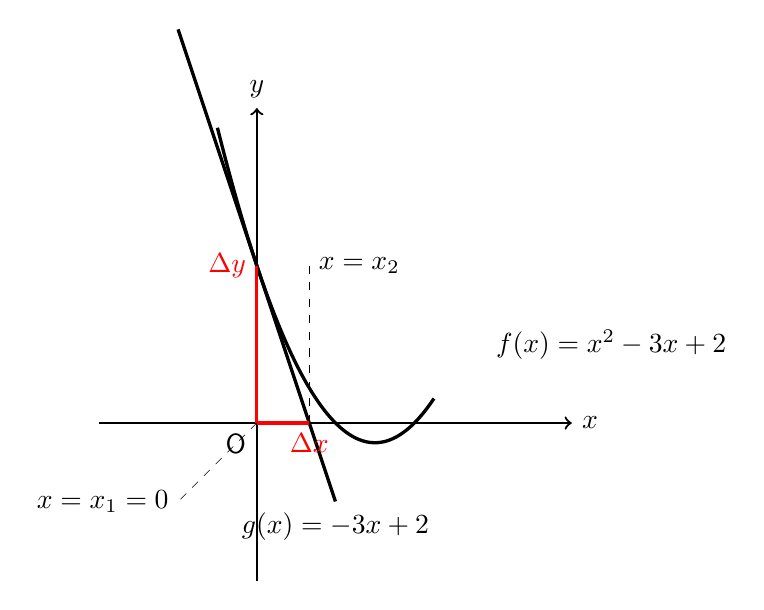
\begin{tikzpicture}[domain=0:8, samples=100, very thick] % 定義域、点の数、線幅
  \draw (0,0) node[below left]{O}; % 原点、0でも、above, below, left, rightで位置指定
  % 位置指定はanchor=north, south, east, westでも可能
  \draw[thick, ->] (-2,0)--(4,0) node[right] {$x$}; % x軸、[->]で矢印、他に[-stealth]等
  \draw[thick, ->] (0,-2)--(0,4) node[above] {$y$}; % y軸

  \draw plot[domain=-0.5:2.25](\x, {(\x*\x)-(3*\x)+2}) node at (4.5,1) {$f(x)=x^2-3x+2$}; % atでnodeの位置指定
  \draw plot[domain=-1:1](\x, -3*\x+2) node[below] {$g(x)=-3x+2$}; % 多項式

  \draw [very thin, dashed](0.666,0) -- (0.666,2) node[above,right]{$x=x_2$}; % 補助線
  \draw [very thin, dashed](0,0) -- (-1,-1) node[above,left]{$x=x_1=0$}; % 補助線
  \draw [red](0,0) -- (0.666,0) node[below]{$\Delta x$}; % 補助線
  \draw [red](0,0) -- (0,2) node[left]{$\Delta y$}; % 補助線
\end{tikzpicture}
\end{frame}

\begin{frame}{ニュートン法}
  \begin{align}
  f^{\prime}(x_1) &= \frac{\Delta y}{\Delta x} \\
  &= \frac{f(x_1)}{x_1 - x_2} \\
  x_1 - x_2 &= \frac{f(x_1)}{f^{\prime}(x_1)} \\
  x_2 &= x_1 -  \frac{f(x_1)}{f^{\prime}(x_1)}
  \end{align}
\end{frame}

\begin{frame}{ニュートン法}
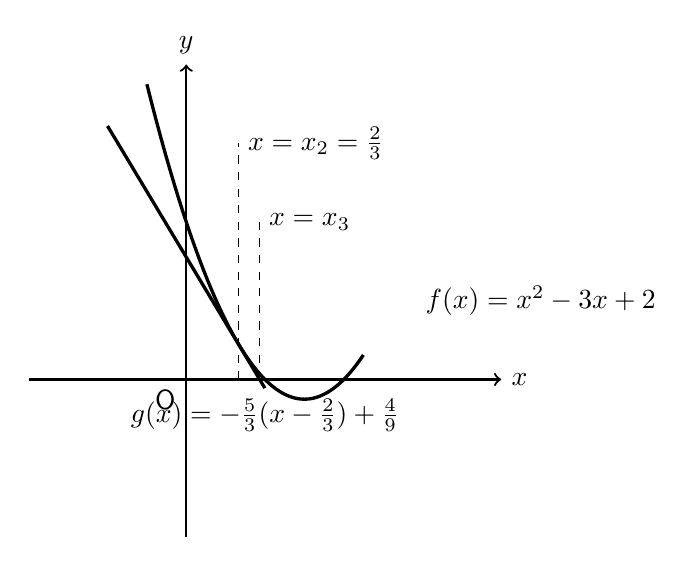
\begin{tikzpicture}[domain=0:8, samples=100, very thick] % 定義域、点の数、線幅
  \draw (0,0) node[below left]{O}; % 原点、0でも、above, below, left, rightで位置指定
  % 位置指定はanchor=north, south, east, westでも可能
  \draw[thick, ->] (-2,0)--(4,0) node[right] {$x$}; % x軸、[->]で矢印、他に[-stealth]等
  \draw[thick, ->] (0,-2)--(0,4) node[above] {$y$}; % y軸

  \draw plot[domain=-0.5:2.25](\x, {(\x*\x)-(3*\x)+2}) node at (4.5,1) {$f(x)=x^2-3x+2$}; % atでnodeの位置指定
  \draw plot[domain=-1:1](\x, {-1.666*(\x-0.666)+0.444}) node[below] {$g(x)=-\frac{5}{3}(x - \frac{2}{3}) + \frac{4}{9}$}; % 多項式
  \draw [very thin, dashed](0.666,0) -- (0.666,3) node[above,right]{$x=x_2=\frac{2}{3}$}; % 補助線
  \draw [very thin, dashed](0.933,0) -- (0.933,2) node[above,right]{$x=x_3$}; % 補助線

\end{tikzpicture}
\end{frame}

\begin{frame}{ニュートン法}
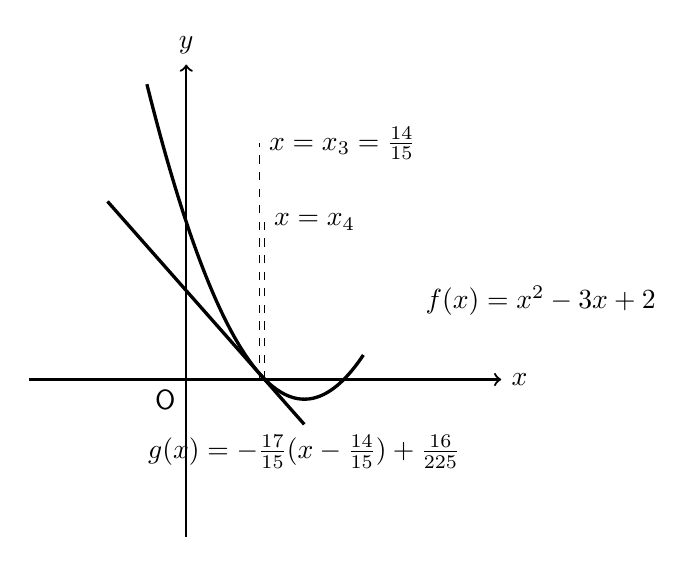
\begin{tikzpicture}[domain=0:8, samples=100, very thick] % 定義域、点の数、線幅
  \draw (0,0) node[below left]{O}; % 原点、0でも、above, below, left, rightで位置指定
  % 位置指定はanchor=north, south, east, westでも可能
  \draw[thick, ->] (-2,0)--(4,0) node[right] {$x$}; % x軸、[->]で矢印、他に[-stealth]等
  \draw[thick, ->] (0,-2)--(0,4) node[above] {$y$}; % y軸

  \draw plot[domain=-0.5:2.25](\x, {(\x*\x)-(3*\x)+2}) node at (4.5,1) {$f(x)=x^2-3x+2$}; % atでnodeの位置指定
  \draw plot[domain=-1:1.5](\x, {-1.133*(\x-0.933)+0.071}) node[below] {$g(x)=-\frac{17}{15}(x - \frac{14}{15}) + \frac{16}{225}$}; % 多項式
  \draw [very thin, dashed](0.996,0) -- (0.996,2) node[above,right]{$x=x_4$}; % 補助線
  \draw [very thin, dashed](0.933,0) -- (0.933,3) node[above,right]{$x=x_3=\frac{14}{15}$}; % 補助線


\end{tikzpicture}
\end{frame}

\begin{frame}{ニュートン法}
\begin{tikzpicture}[domain=0:8, samples=100, very thick] % 定義域、点の数、線幅
  \draw (0,0) node[below left]{O}; % 原点、0でも、above, below, left, rightで位置指定
  % 位置指定はanchor=north, south, east, westでも可能
  \draw[thick, ->] (-2,0)--(4,0) node[right] {$x$}; % x軸、[->]で矢印、他に[-stealth]等
  \draw[thick, ->] (0,-2)--(0,4) node[above] {$y$}; % y軸

  \draw plot[domain=-0.5:2.25](\x, {(\x*\x)-(3*\x)+2}) node at (4.5,1) {$f(x)=x^2-3x+2$}; % atでnodeの位置指定
  \draw [very thin, dashed](0.996,0) -- (0.996,2) node[above,right]{$x=x_4=\frac{254}{255}$}; % 補助線

\end{tikzpicture}
\end{frame}

\begin{frame}{乱数(列)とは}
    出力が一意的ではない数字のこと,法則性がない数列のこと
    \begin{itemize}
      \item 予測不可能性
      \item 一様性
      \item 非周期性
      \item 非再現性
    \end{itemize}
  \end{frame}

  \begin{frame}{予測不可能性}
      \begin{align}
        \vector{x} = \{x_0,x_1,\ldots x_n, \ldots\} \\
        x_{n+1} = ?
      \end{align}
    \end{frame}

    \begin{frame}{一様性}
      \begin{figure}[htbp]
        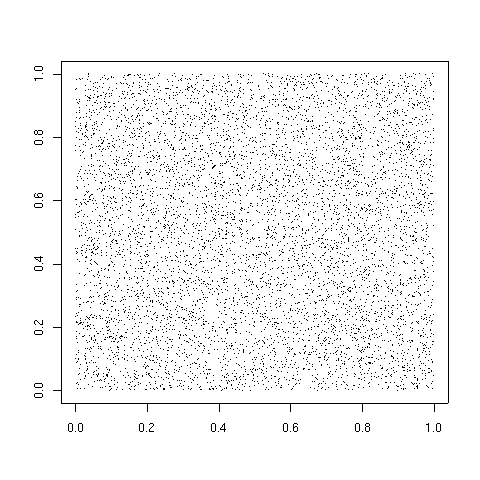
\includegraphics[scale=0.5]{MTrand.png}
      \end{figure}
    \end{frame}

    \begin{frame}{非周期性}
      $f(x + P) = f(x)$となるような$P$は存在しない
    \end{frame}

    \begin{frame}{非再現性}
      $f(\vector{x_0}) \ne f(\vector{x_0})$
    \end{frame}

    \begin{frame}{疑似乱数}
      厳密には決定的であるが乱数列のように見える数列
      \begin{itemize}
        \item 予測不可能性 $\rightarrow$ △
        \item 一様性 $\rightarrow$ △
        \item 非周期性 $\rightarrow$ x
        \item 非再現性 $\rightarrow$ x
      \end{itemize}
    \end{frame}

    \begin{frame}{予測不可能性 $\rightarrow$ △}
      \begin{align}
        \vector{x} &= \{x_0,x_1,\ldots x_n, \ldots\} \\
        x_{n+1} &= (Ax_n + B) \mod M (A,B,M \in \mathbb{Z})
      \end{align}
    \end{frame}

      \begin{frame}{一様性 $\rightarrow$ △}
        \begin{figure}[htbp]
          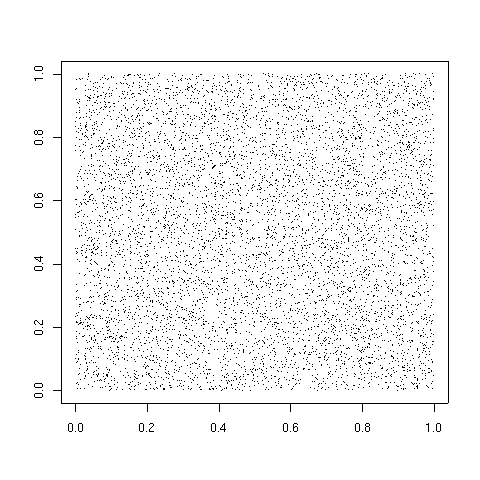
\includegraphics[scale=0.5]{MTrand.png}
        \end{figure}
      \end{frame}

      \begin{frame}{非周期性 $\rightarrow$ x}
        \begin{description}
          \item[線形合同法] $P =2^{32} - 1$
          \item[$n$ビット線形帰還シフトレジスタ] $P = 2^n - 1$
          \item[メルセンヌ・ツイスタ] $P = 2^{19937} - 1$
        \end{description}
      \end{frame}

      \begin{frame}{非再現性 $\rightarrow$ x}
        $f(\vector{x_0}) = f(\vector{x_0})$
      \end{frame}

      \begin{frame}{モンテカルロ積分}
        定積分を乱数を用いた乱択アルゴリズムで解くこと
      \end{frame}

      \begin{frame}{例題}
        \begin{equation}
          \int^1_0 \sqrt{1 - x^2}dx
        \end{equation}
        を解け
        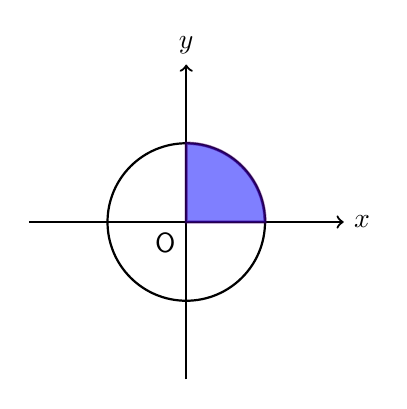
\begin{tikzpicture}[domain=0:8, samples=100, very thick] % 定義域、点の数、線幅
          \draw (0,0) node[below left]{O}; % 原点、0でも、above, below, left, rightで位置指定
          % 位置指定はanchor=north, south, east, westでも可能
          \draw[thick, ->] (-2,0)--(2,0) node[right] {$x$}; % x軸、[->]で矢印、他に[-stealth]等
          \draw[thick, ->] (0,-2)--(0,2) node[above] {$y$}; % y軸

          %\draw plot[domain=-1:1](\x, {sqrt(1-\x^2)}) node[above]{$f(x)=x^2-3x+2$}; % atでnodeの位置指定
          %\draw plot[domain=-1:1](\x, {-sqrt(1-\x^2)}) node[above]{$f(x)=x^2-3x+2$}; % atでnodeの位置指定
          \draw [thick] (0,0) circle (1);
          \filldraw [fill=blue, opacity=.5, draw=Indigo] (1,0)  arc (0:90:1) --(0,0)--cycle;
        \end{tikzpicture}
      \end{frame}

      \begin{frame}
        \begin{align}
          \int^1_0 \sqrt{1 - x^2}dx \\
          \intertext{$x = \cos\theta$と置く}
          \int^{\frac{\pi}{2}}_0 \sqrt{1 - \cos^2\theta} dx \\
          \intertext{$dx = -\sin\theta d\theta$より}
          \int^{\frac{\pi}{2}}_0 \sqrt{1 - \cos^2\theta}(-\sin\theta) d\theta
        \end{align}
      \end{frame}

      \begin{frame}
        \begin{align}
          -\int^{\frac{\pi}{2}}_0 \sin^2\theta d\theta \\
          \intertext{半角の公式より}
          -\frac{1}{2}\int^{\frac{\pi}{2}}_0 1 - 2\cos2\theta d\theta \\
          &= -\frac{1}{2}[\theta + \sin2\theta]^{\frac{\pi}{2}}_0 \\
          &= \frac{\pi}{4}
        \end{align}
      \end{frame}

      \begin{frame}
        計算機で不定積分を介しての解答は不可能(えっ,wolfr(ry) \\
        だけど...
      \end{frame}

      \begin{frame}
        区分求積法というものがある.
      \end{frame}

      \begin{frame}{区分求積法}
        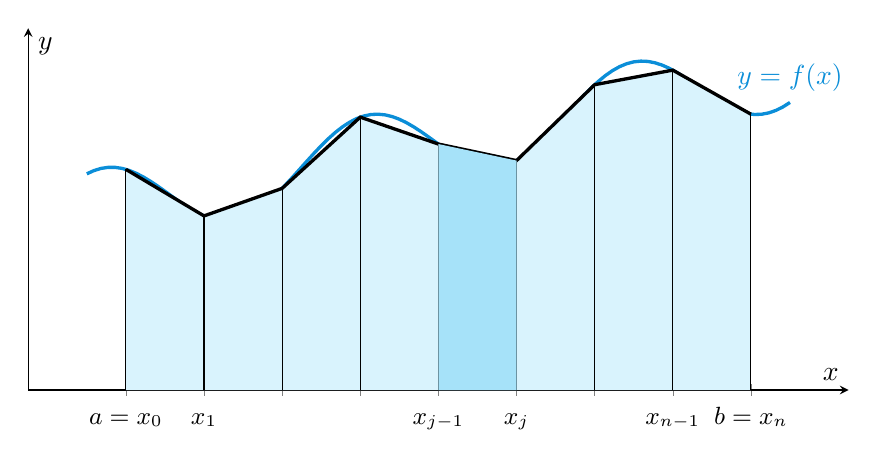
\begin{tikzpicture}[declare function={f=x/5-cos(deg(x*1.85))/2+2;}]
          \begin{axis}[
            integral axis,
            ymin=0,
            xmin=0.75, xmax=11.25,
            domain=1.5:10.5,
            xtick={2,...,10},
            xticklabels={$a=x_0$, $x_1$,,,$x_{j-1}$,$x_j$,,$x_{n-1}$,$b=x_n$},
            ]
            % The function
            \addplot [very thick, cyan!75!blue] {f} node [anchor=south] {$y=f(x)$};

            % The filled area under the approximate integral
            \addplot [integral fill=cyan!15] {f} \closedcycle;

            % The approximate integral
            \addplot [integral line=black] {f};

            % The vertical lines between the segments
            \addplot [integral, ycomb] {f};

            % The highlighted segment
            \addplot [integral fill=cyan!35, domain=6:7, samples=2] {f} \closedcycle;
          \end{axis}
        \end{tikzpicture}
      \end{frame}

      \begin{frame}
        区分求積法なら計算機で計算できる. \\
        モンテカルロ積分の存在意義は? \\
        \pause
        $\rightarrow$ 重積分
      \end{frame}

      \begin{frame}{モンテカルロ積分}
        \begin{tikzpicture}[declare function = {Circle(\x)= sqrt(5-\x)*sqrt(5+\x);}]
          \draw [] (0,0) rectangle (5,5);
          \draw [] (0,5)  arc (180:120:0.5);
          \draw [] (5,5)  arc (0:45:0.5);
          \draw (2.5,5.5) node {2};
          \draw [] (5,0)  arc (0:90:5) --(0,0)--cycle;
          \foreach \i in {1,...,2}
          {
            \foreach \j in {1,...,10}
            {
             \pgfmathsetmacro\myX{random(0,4) + random(0,1000)/1000}%
             \pgfmathsetmacro\myY{random(0,4) + random(0,1000)/1000}%
             \pgfmathsetmacro{\rndcolor}{ Circle(\myX)<\myY ? "red" : "blue" }
             \filldraw[fill=\rndcolor] (\myX, \myY) circle [radius=0.05];            }
            \pause
          }
          \draw (9,5) node {青い点数 = $m$};
          \draw (9,4) node {赤い点数 = $n$};
          \draw (9,3) node {全体的な面積 = $2 \times 2 = 4$};
          \draw (9,2) node {求めたい面積 = $x$};
          \draw (9,1) node {$m : n \approx x : 4$};
        \end{tikzpicture}
      \end{frame}

      \begin{frame}
        $\mathbb{abcdefghijklmnopqrstuvwxyz}$ \\
        $\mathbb{ABCDEFGHIJKLMNOPQRSTUVWXYZ}$ \\
        $\mathbb{1234567890}$ \\
        $\mathbb{<>+-/*}$
      \end{frame}
\end{document}
